%!TEX root = pixelrnn.tex
\section{Introduction}

Generative image modeling is a central problem in unsupervised learning. Probabilistic density models can be used for a wide variety of tasks that range from image compression and forms of reconstruction such as image inpainting (e.g., see Figure \ref{fig:intro_completions}) and deblurring, to generation of new images. When the model is conditioned on external information, possible applications also include creating images based on text descriptions or simulating future frames in a planning task. One of the great advantages in generative modeling is that there are practically endless amounts of image data available to learn from. However, because images are high dimensional and highly structured, estimating the distribution of natural images is extremely challenging.

\begin{figure}[!t]
\centering
\small
\hspace{0.02cm} {occluded} \hfill completions \hfill{original} \,

\vspace{0.1cm}
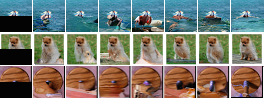
\includegraphics[ width=0.98\linewidth]{compl3.png} %{0 67 133 34}
\vspace{-0.3cm}
\caption{Image completions sampled from a PixelRNN.}
\label{fig:intro_completions}
\vspace{-0.5cm}
\end{figure}

One of the most important obstacles in generative modeling is building complex and expressive models that are also tractable and scalable. This trade-off has resulted in a large variety of generative models, each having their advantages. Most work focuses on stochastic latent variable models such as VAE's \cite{rezende2014stochastic, DBLP:journals/corr/KingmaW13} that aim to extract meaningful representations, but often come with an intractable inference step that can hinder their performance.

One effective approach to \emph{tractably} model a joint distribution of the pixels in the image is to cast it as a product of conditional distributions; this approach has been adopted in autoregressive models such as NADE \cite{larochelle2011} and fully visible neural networks \cite{neal1992connectionist, Bengio_Bengio_NIPS99}. The factorization turns the joint modeling problem into a sequence problem, where one learns to predict the next pixel given all the previously generated pixels. But to model the highly nonlinear and long-range correlations between pixels and the complex conditional distributions that result, a highly expressive sequence model is necessary.

Recurrent Neural Networks (RNN) are powerful models that offer a compact, shared parametrization of a series of conditional distributions. RNNs have been shown to excel at hard sequence problems ranging from handwriting generation \cite{DBLP:journals/corr/Graves13}, to character prediction \cite{sutskever2011generating} and to machine translation \cite{kalchbrenner13emnlp}. A two-dimensional RNN has produced very promising results in modeling grayscale images and textures \cite{theis2015generative}. 

\begin{figure}[h]

% \centering
% 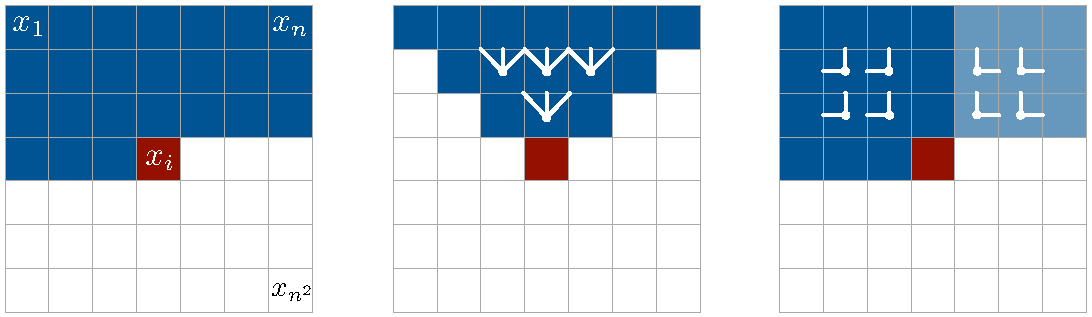
\includegraphics[width=0.48\textwidth]{receptivefields6.pdf}
% \caption{Left: To generate pixel $x_i$ one conditions on all the previously generated pixels left and above of $x_i$. Center: Illustration of a Row LSTM with a kernel of size 3. The dependency field of the Row LSTM does not reach pixels further away on the sides of the image. Right: Illustration of the two directions of the Diagonal BiLSTM. The dependency field of the Diagonal BiLSTM covers the entire available context in the image.}
% \label{depen}
\hfill
\begin{subfigure}{.14\textwidth}
	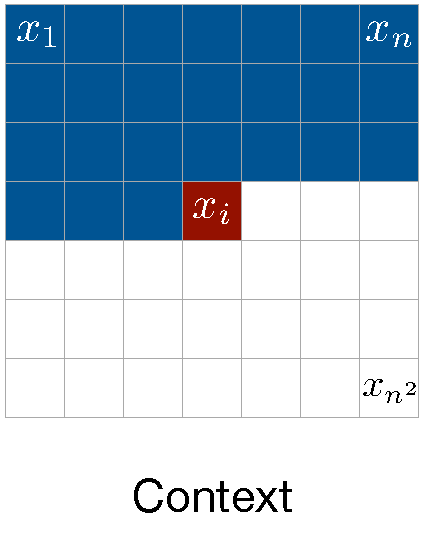
\includegraphics[width=\textwidth]{context5.pdf}
\end{subfigure}
\hfill
\begin{subfigure}{.14\textwidth}
	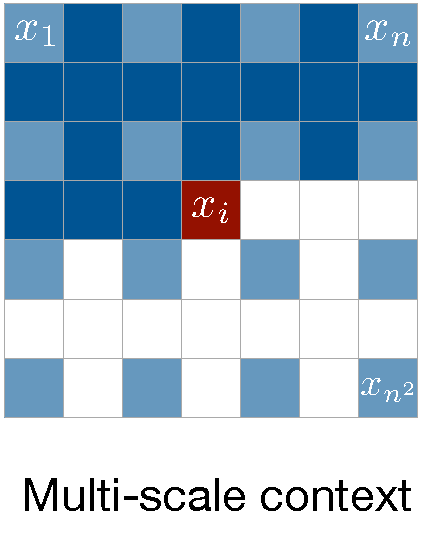
\includegraphics[width=\textwidth]{multiscalecontext.pdf}
\end{subfigure}
\hfill
\begin{subfigure}{.16\textwidth}
	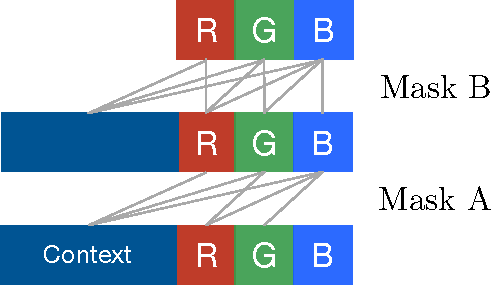
\includegraphics[width=\textwidth]{rgb3.pdf}
\end{subfigure}
\hfill
\caption{\textbf{Left}: To generate pixel $x_i$ one conditions on all the previously generated pixels left and above of $x_i$. \textbf{Center}: To generate a pixel in the multi-scale case we can also condition on the subsampled image pixels (in light blue). \textbf{Right}: Diagram of the connectivity inside a masked convolution. In the first layer, each of the RGB channels is connected to previous channels and to the context, but is not connected to itself. In subsequent layers, the channels are also connected to themselves.}
% \label{fig:residual_and_masking}
\vspace{-0.2cm}
\label{depen}

\end{figure}

In this paper we advance two-dimensional RNNs and apply them to large-scale modeling of natural images.
The resulting \emph{PixelRNNs} are composed of up to twelve, fast two-dimensional Long Short-Term Memory (LSTM) layers. These layers use LSTM units in their state \cite{hochreiter1997long, graves2009offline}  and adopt a convolution to compute at once all the states along one of the spatial dimensions of the data. We design two types of these layers. The first type is the \emph{Row LSTM} layer where the convolution is applied along each row; a similar technique is described in \cite{NIPS2015_5642}. The second type is the \emph{Diagonal BiLSTM} layer where the convolution is applied in a novel fashion along the diagonals of the image. The networks also incorporate \emph{residual connections} \cite{DBLP:journals/corr/HeZRS15} around LSTM layers; we observe that this helps with training of the PixelRNN for up to twelve layers of depth. 

We also consider a second, simplified architecture which shares the same core components as the PixelRNN. 
We observe that Convolutional Neural Networks (CNN) can also be used as sequence model with a fixed dependency range, by using \emph{Masked} convolutions. The \emph{PixelCNN} architecture is a fully convolutional network of fifteen layers that preserves the spatial resolution of its input throughout the layers and outputs a conditional distribution at each location.
 
Both PixelRNN and PixelCNN capture the full generality of pixel inter-dependencies without introducing independence assumptions as in e.g., latent variable models. The dependencies are also maintained between the RGB color values within each individual pixel. 
Furthermore, in contrast to previous approaches that model the pixels as continuous values (e.g., \citet{theis2015generative, gregor2013deep}), we model the pixels as \emph{discrete} values using a multinomial distribution implemented with a simple softmax layer. We observe that this approach gives both representational and training advantages for our models.


The contributions of the paper are as follows. In Section \ref{sect:pixelrnn} we design two types of PixelRNNs corresponding to the two types of LSTM layers; we describe the purely convolutional PixelCNN that is our fastest architecture; and we design a \emph{Multi-Scale} version of the PixelRNN.
In Section \ref{sect:experiments} we show the relative benefits of using the discrete softmax distribution in our models and of adopting residual connections for the LSTM layers. Next we test the models on MNIST and on CIFAR-10 and show that they obtain log-likelihood scores that are considerably better than previous results. We also provide results for the large-scale ImageNet dataset resized to both $32 \times 32$ and $64 \times 64$ pixels; to our knowledge likelihood values from generative models have not previously been reported on this dataset. Finally, we give a qualitative evaluation of the samples generated from the PixelRNNs. %The samples are crisp, give evidence of significant object and scene awareness and create realistic novel compositions.


